\nsection{Problem 1 - (Simulation from 1D distribution)}
We will start this exercise by investigating some
methods for sampling a univariate distribution. We will assume that we easily obtain samples
from a uniform distribution, i.e. $U \sim \text{Unif}[0,1]$
\nssection{a.)}
\emph{Describe the standard transformation rule to sample from a univariate distribution, and
derive the expression for sampling from an exponential distribution.} \spaze 
\textbf{Solution:} \spaze
Initially we assume to draw a sample $U$ from a uniform distribution $\text{Unif}[0,1]$. Then we turn to the target distribution given by 
\begin{align*}
    F(x) = \int_{-\infty}^{x} f(u) \ du
\end{align*}
whereby looking at the inverse of $f(x)$ will transform the uniform sample $U$ into a sample from our desired distribution. Namely 
\begin{align*}
    X = F^{-1}(U) = \inf \bl x \mid F(x) \geq u \br
\end{align*}
where $\inf \bl x \mid F(x) \geq u \br$ is well-known from inverse transform sampling and that $F$ is right-continuous, meaning $\bl u \mid F(x) \geq u \br$ is well-defined. 

Suppose so that $X \sim \text{Exp}(\lambda)$. We know that $f(x) = \lambda e^{-\lambda x}$, for $x \geq 0 $ and accordingly $F(x) = 1 - e^{-\lambda x}$, which by application of the transformation yields 
\begin{align*}
F(x) = U \\[5pt]
1 - e^{-\lambda x} = U \\[5pt] 
e^{-\lambda x} = 1 - U  \\[5pt]
-\lambda x = \ln(1 - U) \\[5pt]
x = -\frac{\ln(1 - U)}{\lambda} 
\end{align*}
Meaning our sample transformation gives $\boxed{x = -\frac{\ln(1 - U)}{\lambda}}$, and we are done. $\Q$
\nssection{b.)}
\emph{When the negative log density is convex we can use adaptive rejection sampling to build an
approximation to the density. We will now use this to sample from a standard normal
distribution. We shall use the sub-gradient of the convex function, i.e. for a continuously
differentiable convex function $k(x)$ we have:} 
\begin{align*}
    k(x) \geq k(x_0) + k^{\prime}(x_0)(x - x_0)
\end{align*}
\emph{Describe how we can use the convex property of the negative log density to find an
upper bound on the distribution. Use the linearization around the points -1, 0, and 1,
to derive a bounding function for the standard normal. Illustrate the bounding function.
Does the bounding function integrate to 1? Show that the probability distribution
corresponding to the bounding function is:} 
\begin{align}
g(x) = 
\begin{cases}
    \frac{1}{3} & \text{if } -0.5 < x \leq 0.5 \\[5pt]
    \frac{\exp(-|x| + 0.5)}{3} & \text{else}
\end{cases} \label{eq:prop_exer_1}
\end{align}
\textbf{Solution:} \spaze 
\underline{\textbf{Upper Bound:}}

Suppose we have found the log-density of some data $x$, which we denote by $\ell(x)$. Now since $-\ell(x)$ is convex we have from the result of the sub-gradient that 
\begin{align*}
    -\ell(x) &\geq -\ell(x_0) - \ell^{\prime}(x_0)(x - x_0) \\[5pt]
    & \hspace{1cm} \Updownarrow \\[5pt]
    \ell(x) &\leq \ell(x_0) + \ell^{\prime}(x_0)(x - x_0)
\end{align*}
where reversing the log-transformation gives 
\begin{align}
    e^{\ell(x)} \leq e^{\ell(x_0) + \ell^{\prime}(x_0)(x - x_0)}.
\end{align}
This is nothing more than a description of the limitation to the likelihood density function, meaning 
\begin{align*}
    L(x) \leq e^{\ell(x_0) + \ell^{\prime}(x_0)(x - x_0)}
\end{align*}
whereby taking the minimum of the right hand side over several points would yield a sensible upper bound 
\begin{align}
    L(x) \leq \min \bl e^{\ell(x_i) + \ell^{\prime}(x_i)(x - x_i)} \br
\end{align}
\underline{\textbf{Linearization:}}

We start off by computing $\ell(x)$
\begin{align*}
    \ell(x) &= \log \left( \phi(x) \right) \\[5pt]
    &= \log \left(\frac{1}{\sqrt{2\pi}}e^{-\frac{x^2}{2}} \right) \\[5pt] 
    &= \log \left( \frac{1}{\sqrt{2 \pi}} \right) - \frac{x^2}{2}
\end{align*}
and then $\ell^{\prime}(x)$  
\begin{align*}
    \ell^{\prime}(x) = -x
\end{align*}
\textbf{Case 1:} $x = -1$

By linearization we have that 
\begin{align}
    \mathcal{B}(x) &= \ell(-1) + \ell^{\prime}(-1)(x - (-1)) \\[5pt]
        &= \log \left( \frac{1}{\sqrt{2 \pi}} \right) - \frac{1}{2} + 1 \cdot(x -(-1)) \\[5pt]
        &= \log \left( \frac{1}{\sqrt{2 \pi}} \right) + x + \frac{1}{2}
\end{align}
\textbf{Case 2:} $x = 0$

In like manner 
\begin{align}
    \mathcal{B}(x) &= \ell(0) + \ell^{\prime}(0)(x) \\[5pt]
        &= \log \left( \frac{1}{\sqrt{2 \pi}} \right) - 0\\[5pt]
        &= \log \left( \frac{1}{\sqrt{2 \pi}} \right)
\end{align}
\textbf{Case 3:} $x = 1$

And lastly 
\begin{align}
    \mathcal{B}(x) &= \ell(1) + \ell^{\prime}(1)(x - 1) \\[5pt]
        &= \log \left( \frac{1}{\sqrt{2 \pi}} \right) - \frac{1}{2} - 1 \cdot(x - 1) \\[5pt]
        &= \log \left( \frac{1}{\sqrt{2 \pi}} \right) - x + \frac{1}{2}
\end{align}
Additionally it is worth nothing that the three resulting linearization lines intercept each other in $x_1 = -\frac{1}{2}, x_2 = 0$ and $x_3 = \frac{1}{2}$ respectively. Which then gives us the following bounding function 
\begin{align}
    \mathcal{B}(x) = \begin{cases}
        \log \left( \frac{1}{\sqrt{2 \pi}} \right) + x + \frac{1}{2}, \ &x \in (-\infty, -\frac{1}{2}) \\[5pt]
        \log \left( \frac{1}{\sqrt{2 \pi}} \right) \ &x \in [-\frac{1}{2}, \frac{1}{2}) \\[5pt]
        \log \left( \frac{1}{\sqrt{2 \pi}} \right) - x + \frac{1}{2}, \ &x \in [\frac{1}{2}, \infty)
    \end{cases}
\end{align}
and is illustrated in the plot below, produced by the code in Appendix (\ref{appendix:b}), from code listings (\ref{lst:boundary_func})
\begin{figure}[H]
    \centering
    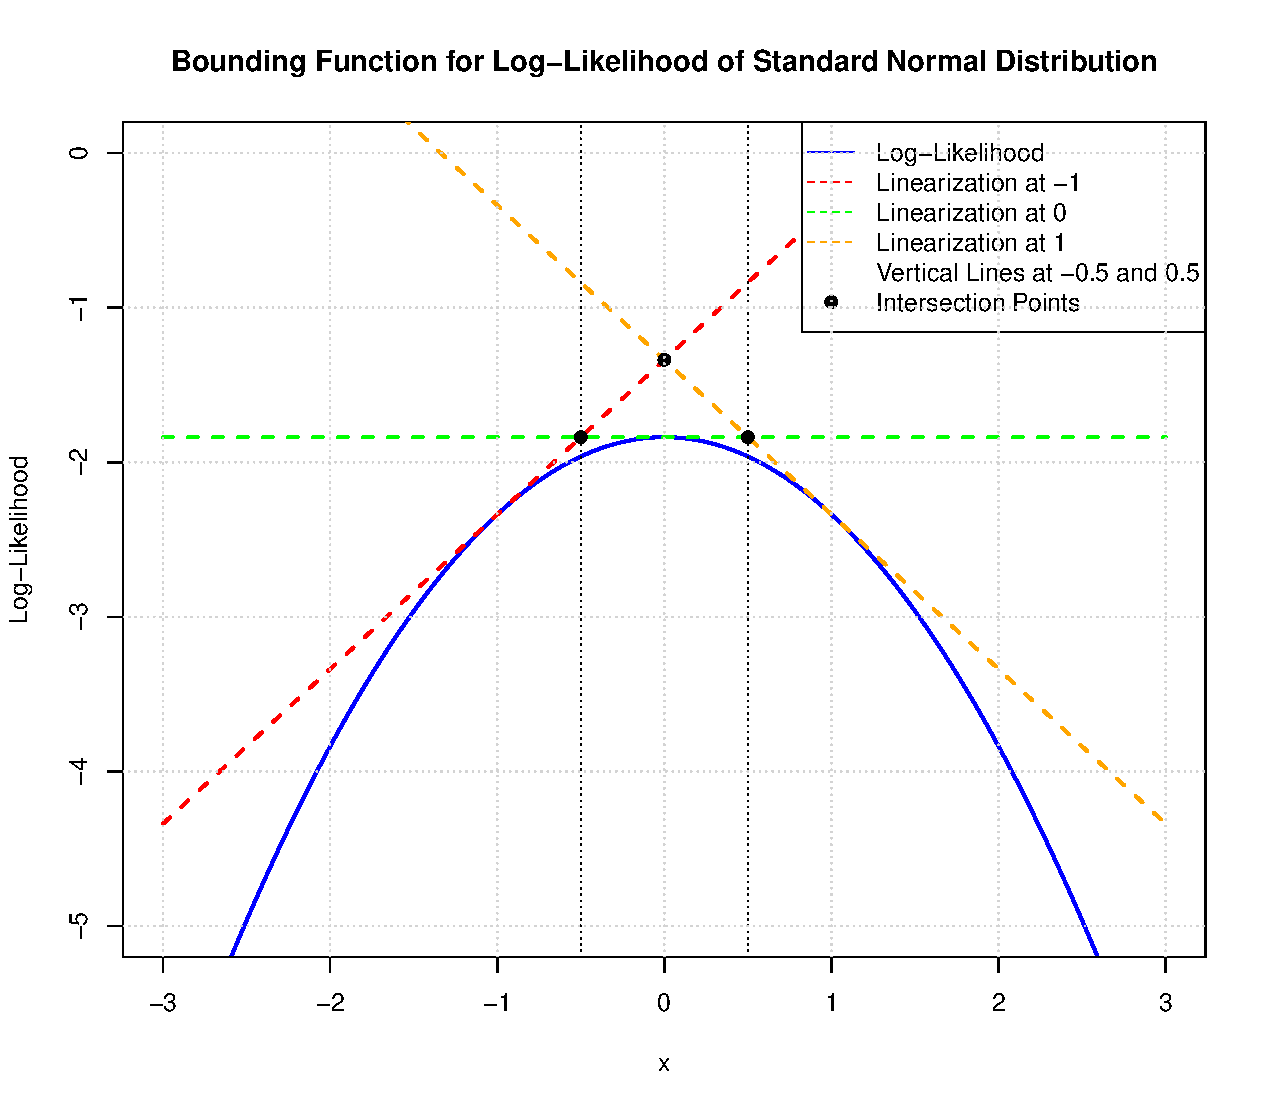
\includegraphics[width=0.8\textwidth]{Images/Exercise_1_Figures/Boundary_func.pdf} 
    \caption{Illustration of the boundaries for the log-density, with the linearization lines and their respective points of intersection.}
    \label{fig:example}
\end{figure}
When integrating $\mathcal{B}(x)$ we observe that the resulting improper integrals are tedious to analyse, but by exponentially transforming $\mathcal{B}(x)$ (i.e $e^{\mathcal{B}(x)}$) the task becomes rather straightforward. We proceed
\begin{align*}
    \mathcal{G}(x) &= e^{\mathcal{B}(x)} \\[5pt]
    &= \begin{cases}
         \frac{1}{\sqrt{2 \pi}} \left( e^{x + \frac{1}{2}} \right), \ &x \in (-\infty, -\frac{1}{2}) \\[5pt]
        \frac{1}{\sqrt{2 \pi}}\ &x \in [-\frac{1}{2}, \frac{1}{2}) \\[5pt]
        \frac{1}{\sqrt{2 \pi}} \left( e^{- x + \frac{1}{2}} \right), \ &x \in [\frac{1}{2}, \infty)
    \end{cases} \\[15pt]
    &=  \frac{1}{\sqrt{2 \pi}} \begin{cases}
         e^{x + \frac{1}{2}} , \ &x \in (-\infty, -\frac{1}{2}) \\[5pt]
        1 \ &x \in [-\frac{1}{2}, \frac{1}{2}) \\[5pt]
         e^{- x + \frac{1}{2}}, \ &x \in [\frac{1}{2}, \infty)
    \end{cases}
\end{align*}
where then the integral of $\mathcal{G}(x)$ becomes 
\begin{align*}
    \int_{-\infty}^{\infty} \mathcal{G}(x) &= \frac{1}{\sqrt{2 \pi}} \left( \int_{-\infty}^{-1/2} e^{x + \frac{1}{2}} \ dx + \int_{-1/2}^{1/2} 1 \ dx + \int_{1/2}^{\infty}  e^{- x + \frac{1}{2}}  \ dx\right) \\[8pt]
    &= \frac{1}{\sqrt{2 \pi}} \left( \left[e^{x + \frac{1}{2}}\right]_{-\infty}^{-\frac{1}{2}} + 1 + \left[- e^{-x + \frac{1}{2}}\right]_{\frac{1}{2}}^{\infty} \right) \\[7pt]
    &= \frac{1}{\sqrt{2 \pi}} \left( 1 + 1 + 1\right) \\[7pt]
    &= \frac{3}{\sqrt{2 \pi}}
\end{align*} 
which is not equal to 1. 

Since the bounding function $\mathcal{G}(x)$ did not integrate to $1$ we recall from rudimentary probability theory that if we are to find the probability distribution of $\mathcal{G}(x)$ then its integral must equate to $1$. This can be done by letting 
\begin{align*}
    g(x) = k\mathcal{G}(x)
\end{align*}
for some sufficient $k \in \mathbb{R}$ satisfying the criterion. Where in this case $k = \frac{\sqrt{2 \pi}}{3}$, which gives 
\begin{align*}
    g(x) &= \frac{\sqrt{2 \pi}}{3} \cdot \mathcal{G}(x) \\[5pt]
    &= \begin{cases}
         \frac{e^{x + \frac{1}{2}}}{3} , \ &x \in (-\infty, -\frac{1}{2}) \\[5pt]
        \frac{1}{3} \ &x \in [-\frac{1}{2}, \frac{1}{2}) \\[5pt]
         \frac{e^{- x + \frac{1}{2}}}{3}, \ &x \in [\frac{1}{2}, \infty)
    \end{cases} \\[15pt]
    &= \begin{cases}
    \frac{1}{3} & \text{if } -0.5 < x \leq 0.5 \\[5pt]
    \frac{\exp(-|x| + 0.5)}{3} & \text{else}
\end{cases}
\end{align*}
and we are done. $\Q$
\nssection{c.)}
\emph{Algorithm 1 below uses rejection sampling to sample the standard normal distribution.
Show the relation to the distribution in (\ref{eq:prop_exer_1}), compute the average acceptance rate, and
implement the algorithm} \spaze 
\begin{algorithm}[H]
\SetAlgoLined
\KwResult{Accepted sample $x_p$}
\While{not accepted}{
    Sample $U_1, U_2$ iid from $\text{Unif}[0,1]$\;
    Sample $i \in \{1,2,3\}$, with probability $p_0=\left\{\frac{1}{3}, \frac{1}{3}, \frac{1}{3}\right\}$\;
    \eIf{$i = 1$}{
        $x_p = U_1 - 0.5$\;
    }{
        \eIf{$i = 2$}{
            $x_p = \ln(1 - U_1) - 0.5$\;
        }{
            $x_p = -\ln(1 - U_1) + 0.5$\;
        }
    }
    \If{$U_2 < \frac{\sqrt{2\pi} \cdot \phi(x_p)}{3 \cdot g(x_p)}$}{
        Accept proposal and return $x_p$\;
    }
}
\caption{Rejection Sampling Algorithm}
\end{algorithm}
\textbf{Solution:} \spaze 
We start off by finding the relation between the sampling algorithm and $g(x)$ through inverse transform sampling, like it is sketched in (a.). 

\textbf{Finding the cumulative distribution function (CDF):}

The first step in our transformation involves finding $G(x)$, which is simply to look at 
\begin{align}
    G(x) &= \frac{1}{3} \left(\int_{-\infty}^{-1/2} e^{x + \frac{1}{2}} \ dx \right) , \ \text{ for } x \in (-\infty, -\frac{1}{2}] \\[5pt]
    G(x) &=  \frac{1}{3} \left(\int_{-\infty}^{-0.5} e^{x + \frac{1}{2}}  + \int_{-0.5}^{x} 1 \ dx \right) , \ \text{ for } x \in (-\frac{1}{2}, \frac{1}{2}] \\[5pt] 
     G(x) &=  \frac{1}{3} \left(\int_{-\infty}^{-1/2} e^{x + \frac{1}{2}}  + \int_{-1/2}^{1/2} 1 \ dx + \int_{1/2}^{\infty} e^{-x + \frac{1}{2}} \right) , \ \text{ for } x \in (\frac{1}{2}, \infty)
\end{align}
where by doing these calculations give us the following CDF 
\begin{align*}
    G(x) = \begin{cases}
         \frac{e^{x + \frac{1}{2}}}{3} , \ &x \in (-\infty, -\frac{1}{2}]\\[5pt]
        \frac{1}{3} + \frac{x + 0.5}{3}\ &x \in (-\frac{1}{2}, \frac{1}{2}] \\[5pt]
         1 - \frac{e^{- x + \frac{1}{2}}}{3}, \ &x \in (\frac{1}{2}, \infty)
    \end{cases}
\end{align*}
\textbf{Inverse transformation:}

The next step is hence to find the inverse of $G(x)$, which again must be done to each separate argument in $G(x)$ 
\begin{align}
    G^{-1}(y) &= \log(3y) - \frac{1}{2}, \ \text{ for } y \in(0, \frac{1}{3}] \\[5pt]
    G^{-1}(y) &= 3y - \frac{3}{2}, \ \text{ for } y \in(\frac{1}{3}, \frac{2}{3}] \\[5pt]
    G^{-1}(y) &= -\log(-3y +3) + \frac{1}{2}, \ \text{ for } y \in(\frac{2}{3}, 1).
\end{align}
The inverse variable $y$ now spans from $0$ to $1$ which tells us that we are in the correct domain of sampling. The full inverse is then expressed as 
\begin{align*}
    G^{-1}(y) = \begin{cases}
        \log(3y) - \frac{1}{2}, \  &y \in(0, \frac{1}{3}] \\[5pt]
         3y - \frac{3}{2}, \  &y \in(\frac{1}{3}, \frac{2}{3}] \\[5pt]
         -\log(-3y +3) + \frac{1}{2}, \ &y \in(\frac{2}{3}, 1)
    \end{cases}
\end{align*}
and if by substituting $u = 3y$ yields 
\begin{align*}
      G^{-1}(u) = \begin{cases}
        \log(u) - \frac{1}{2}, \  &y \in(0, 1] \\[5pt]
         u - \frac{3}{2}, \  &y \in(1, 2] \\[5pt]
         -\log(-u +3) + \frac{1}{2}, \ &y \in(2, 3)
    \end{cases}
\end{align*}
making $U \sim \text{Unif}[0, 3]$. 

The implementation of the rejection sampling scheme can be found in Appendix (\ref{appendix:b}), from code listings (\ref{lst:rejection}) and produces the following output for our acceptance rate: 
\begin{align*}
    U_{\text{rate}} = 0.8358 \approx \frac{\sqrt{2 \pi}}{3}
\end{align*}
\nssection{d.)}
\emph{An alternative to rejection sampling is importance sampling. Implement an importance
sampler based on $g(x)$. Give arguments for choices you make when setting up the
importance sampler.} \spaze 
\textbf{Solution:} \spaze
The implementation of the importance sampling algorithm can be found in Appendix (\ref{appendix:b}), from code listings (\ref{lst:importance}) and produces the following output
\begin{align*}
    \hat{\mathbb{E}}(g) = 0.497625803124113
\end{align*}
 In importance sampling, we aim to estimate properties of a \textbf{target} distribution by drawing samples from a \textbf{proposal} distribution, and assigning weights to each sample based on their likelihood under the target distribution compared to the proposal distribution. Important considerations can include choosing a proposal distribution with heavier tails than the target distribution, making sure there is coverage of the entire target distribution to avoid zero probabilities, normalizing weights to ensure they sum to 1, and estimating the desired property by computing a weighted average of the samples. The number of samples to generate depends on the desired accuracy of the estimate.
\nssection{e.)}
\emph{Discuss the differences between rejection sampling and importance sampling.
Compare the two approaches in a numerical study where you quantify the Monte Carlo variance in the results. For each rerun of the estimation should be based on 1000
samples from $g(x)$. In the numerical study you should estimate $\mathbb{E}(h(x))$, where:}
\begin{align*}
    h(x) = x^2 I(x > 0)
\end{align*}
\textbf{Solution:} \spaze
The implementation of the numerical comparison can be found in Appendix (\ref{appendix:b}), from code listings (\ref{lst:compare}) and produces the following output: 
\begin{align*}
    \hat{\mathbb{E}}_{\text{RS}}(h) &=  0.526384920450183 \\[5pt]
    \hat{\mathbb{E}}_{\text{IS}}(h) &=  0.487551647399552 \\[10pt]
    \text{SD}_{RS}(h) &=  1.13961507092653 \\[5pt]
     \text{SD}_{IS}(h) &= 0.278753890995243
\end{align*}
where $\hat{\mathbb{E}}_{\text{RS}}(h), \hat{\mathbb{E}}_{\text{IS}}(h)$ are the estimates for the rejection sampling (RS) and importance sampling (IS) respectively. From the results shown above we conclude that importance sampling yield slightly better results than rejection.

\underline{\textbf{Differences:}}

 Rejection sampling involves generating samples from a proposal distribution and accepting or rejecting them based on their likelihood under the target distribution. This method requires a well-defined rejection criterion and may result in low acceptance rates, especially in higher dimensional spaces. Conversely, importance sampling directly estimates properties of the target distribution by weighting samples drawn from a proposal distribution. It provides unbiased estimates, but relies heavily on the choice of proposal distribution, which should cover the entire target distribution (i.e exercise 1d) to avoid significant weights in regions of low probability density. 